\documentclass[11pt,a4,twosided,singlespacing,titlepagenumber=on]{scrreprt}
%%%obsolete starting points. (ignore)
%\documentclass[a4paper,12pt,singlespace,report]{memoir}
%\documentclass[a4,11pt,singlespace,MSc]{icldt}

\usepackage[T1]{fontenc} % Handles accents etc better in the invisible details of the pdf output.
\usepackage[latin1]{inputenc} % May or may not be needed. Says that your *.tex file is a text file with ASCII latin1 encoding. You could use e.g. utf8 instead for easier accents etc.
\usepackage[UKenglish]{babel} % Let LaTeX know what language the text is in so it can select the correct hyphenation pattern etc

%%% American Mathematical Society packages
\usepackage{amsfonts,amssymb,amsmath,amsthm}
\usepackage{amsbsy}

%%% Graphics packages
\usepackage{float}
%\floatstyle{boxed} 
\restylefloat{figure}

\usepackage{graphicx}
%\graphicspath{{figures/}} % Useful if you have lots of images and want to keep thinks tidy by having a subfolder for images
%\usepackage{tikz} %For creating vector-graphics diagrams, flowcharts etc directly in LaTeX (takes some time to learn)
\usepackage[absolute]{textpos} % Used to position the Imperial College logo. You can comment this line and the next line out if you don't use the logo.
\usepackage[table,xcdraw]{xcolor}

%%% Referencing and cross-referencing
\usepackage[colorlinks=false,pdfborder={0 0 0},plainpages=false,pdfpagelabels]{hyperref} % If you click on an item in the table of contents or a referenced equation/figure number, the PDF will go to the desired page. Neat isn't it?
\usepackage[round,authoryear,sort]{natbib} % Enable bibtex-based bibliography generation
%\usepackage[square,numbers,sort&compress]{natbib} % If you want numbered referencing instead of author-year style.

%\setcounter{secnumdepth}{3} %If you want subsubsections to be numbered
\numberwithin{equation}{chapter} % Reset equation numbers after each chapter.

%%%%%%%%%%%%%%%%%%%%%%%%%%%%%%%%%%%%%
%%%%% Define how to create the title page  %%%%%%%%%%%%%%%%
%%%%%%%%%%%%%%%%%%%%%%%%%%%%%%%%%%%%%
\makeatletter
\newcommand*{\supervisor}[1]{\gdef\@supervisor{#1}}
\newcommand*{\CID}[1]{\gdef\@CID{#1}}
\newcommand*{\logoimg}[1]{\gdef\@logoimg{#1}}
\renewcommand{\maketitle}{
\begin{titlepage}
\ifdefined\@logoimg
\begin{textblock*}{8cm}(1.75cm,1.75cm)
\includegraphics[width=70mm]{\@logoimg}
\end{textblock*}
\vspace*{1cm}
\else
%\vspace*{0cm}
\fi
\begin{center}
\vspace*{\stretch{0.1}}
Imperial College London\\
Derpartment of Mathematics\par
\vspace*{\stretch{1}} % This inserts vertical space and allows you to specify a relative size for the vertical spaces.
{\titlefont\Huge \@title\par} % If your title is long, you may wish to use \huge instead of \Huge.
\vspace*{\stretch{2}}
{\Large \@author \par}
\vspace*{1em}
{\large CID: \@CID \par}
\vspace*{\stretch{0.5}}
{\large Supervised by \@supervisor \par}
\vspace*{\stretch{3}}
{\Large \@date \par}
\vspace*{\stretch{1}}
{\large Submitted in partial fulfilment of the requirements for the
MSc in Statistics of Imperial College London}
\vspace*{\stretch{0.1}}
\end{center}%
\end{titlepage}%
}
\makeatother

%%% And the plagiarism declaration
\newcommand*{\declaration}{%
\vspace*{0.3\textheight}
The work contained in this thesis is my own work unless
otherwise stated.\\
\vspace*{0.1\textheight}\\
\hspace*{0.25\textwidth}Signed: \hspace{0.25\textwidth} Date:
\clearpage}

%%% And the abstract page
\renewenvironment{abstract}%
{\chapter*{Abstract}\thispagestyle{plain}}%
{\clearpage}
%%% And why not change the quote environment
\newenvironment{myquote}%
{\begin{quote}{\Large{}``}}%
{\ifhmode\unskip\fi{\Large{}''}\end{quote}}




%%% Actual words used in the title page
\title{Segmentation of CT scans into Atrium/non Atrium}
\author{Thomas Vogel}
\CID{}
\supervisor{Prof Giovanni Montana}
\date{\today}
\logoimg{Imperial__4_colour_process.jpg}

%%%%%%%%%%%%%%%%%%%%%%%%%%%%%%%%%%%%%
%%%%% End of preamble and start of document %%%%%%%%%%%%%%
%%%%%%%%%%%%%%%%%%%%%%%%%%%%%%%%%%%%%

\begin{document}

\maketitle %Generates the Title Page

\declaration %Insert plagiarism statement

\begin{abstract}
This is a \LaTeX{} template to be used for project theses by the students of the Imperial College MSc in Statistics. Please have a look at the \verb|*.tex| source and the code comments therein. You may use this template with only minor changes, or make any major style changes you desire (e.g. redesigning the title page, adding headers,...), or you may use a different template, or you may write your own approach from scratch, or you may just use some bits and pieces from the template's \LaTeX{} code. It's up to you. Note that resources on how to use \LaTeX{} are available on Blackboard under `R\&{}LaTeX intro'.

This template will quote relevant sections from the MSc in Statistics student handbook throughout; e.g.
\begin{myquote}
The abstract should be a brief statement of the aims and outcomes of the project, to summarise/advise
even for a casual reader!
\end{myquote}
\end{abstract}
\newpage
\chapter*{Acknowledgements}
Thank you supervisor/friends/family/pet.
\begin{myquote}
Include an acknowledgement.
\end{myquote}
\newpage

% Automatically create a table of contents
\renewcommand{\contentsname}{Table of Contents}
\tableofcontents
\newpage

% Figure and table lists if you want them.
%\cleardoublepage
%\phantomsection
%\listoffigures 
%\addcontentsline{toc}{chapter}{\listfigurename}
%\newpage
%\phantomsection
%\listoftables  
%\addcontentsline{toc}{chapter}{\listtablename}
%\newpage

\chapter{Background Material: on convolutional neural networks}

A convolutional neural network (CNN) is a specialised kind of feed-forward Neural Network that replaces standard matrix multiplication for a convolution. A convolutional layer has three components: a convolution part, an activation part, and a subsampling/pooling part.

\section{Convolutional Neural Networks}

\subsection{Convolution}

The input is processed by several kernels with learnable weights, each producing a set of outputs called feature maps. This leverages three ideas:

\begin{itemize}
	\item sparse interaction: every output node is connected to a local sub- set of inputs.
	\item parameter sharing: the same kernel is used for every output node in a given feature map.
	\item translational equivariance: shifting the input results in an equiv- alent shift in the output.
\end{itemize}

\subsection{Activation}
Every node in the feature map is passed to an activation function, usually a Tanh unit or a Rectified Linear unit.

\subsection{Subsampling/pooling}

Reduces the output with a local summary statistic, e.g. maximum or average. This reduces the layer size and adds local translational invariance.

\subsection{Typical Architecture}

The architecture considered consists in an input layer which are square patches centred at the voxel of interest, two convolutional layers, a fully connected layer, and an output layer. Each layer in turn represents more abstract features the deeper its location in the architecture.
Compared to a deep multiple layer perceptron, this architecture has the ad- vantage of being memory and computationally efficient.
\chapter{Background Material: on Convolutional Neural Networks}

\noindent We first start with a brief review of feedforward neural networks before elaborating on convolutional neural networks (CNNs). A number of good books available expand on the following content in much greater detail, notably \citep{Bengio-et-al-2015-Book}, \citep{Bishop:1995:NNP:525960} and \citep{Nielsen}.

\section{Feed Forward Neural Networks}

\begin{figure}
\centering
\label{Basic_neural_network}
%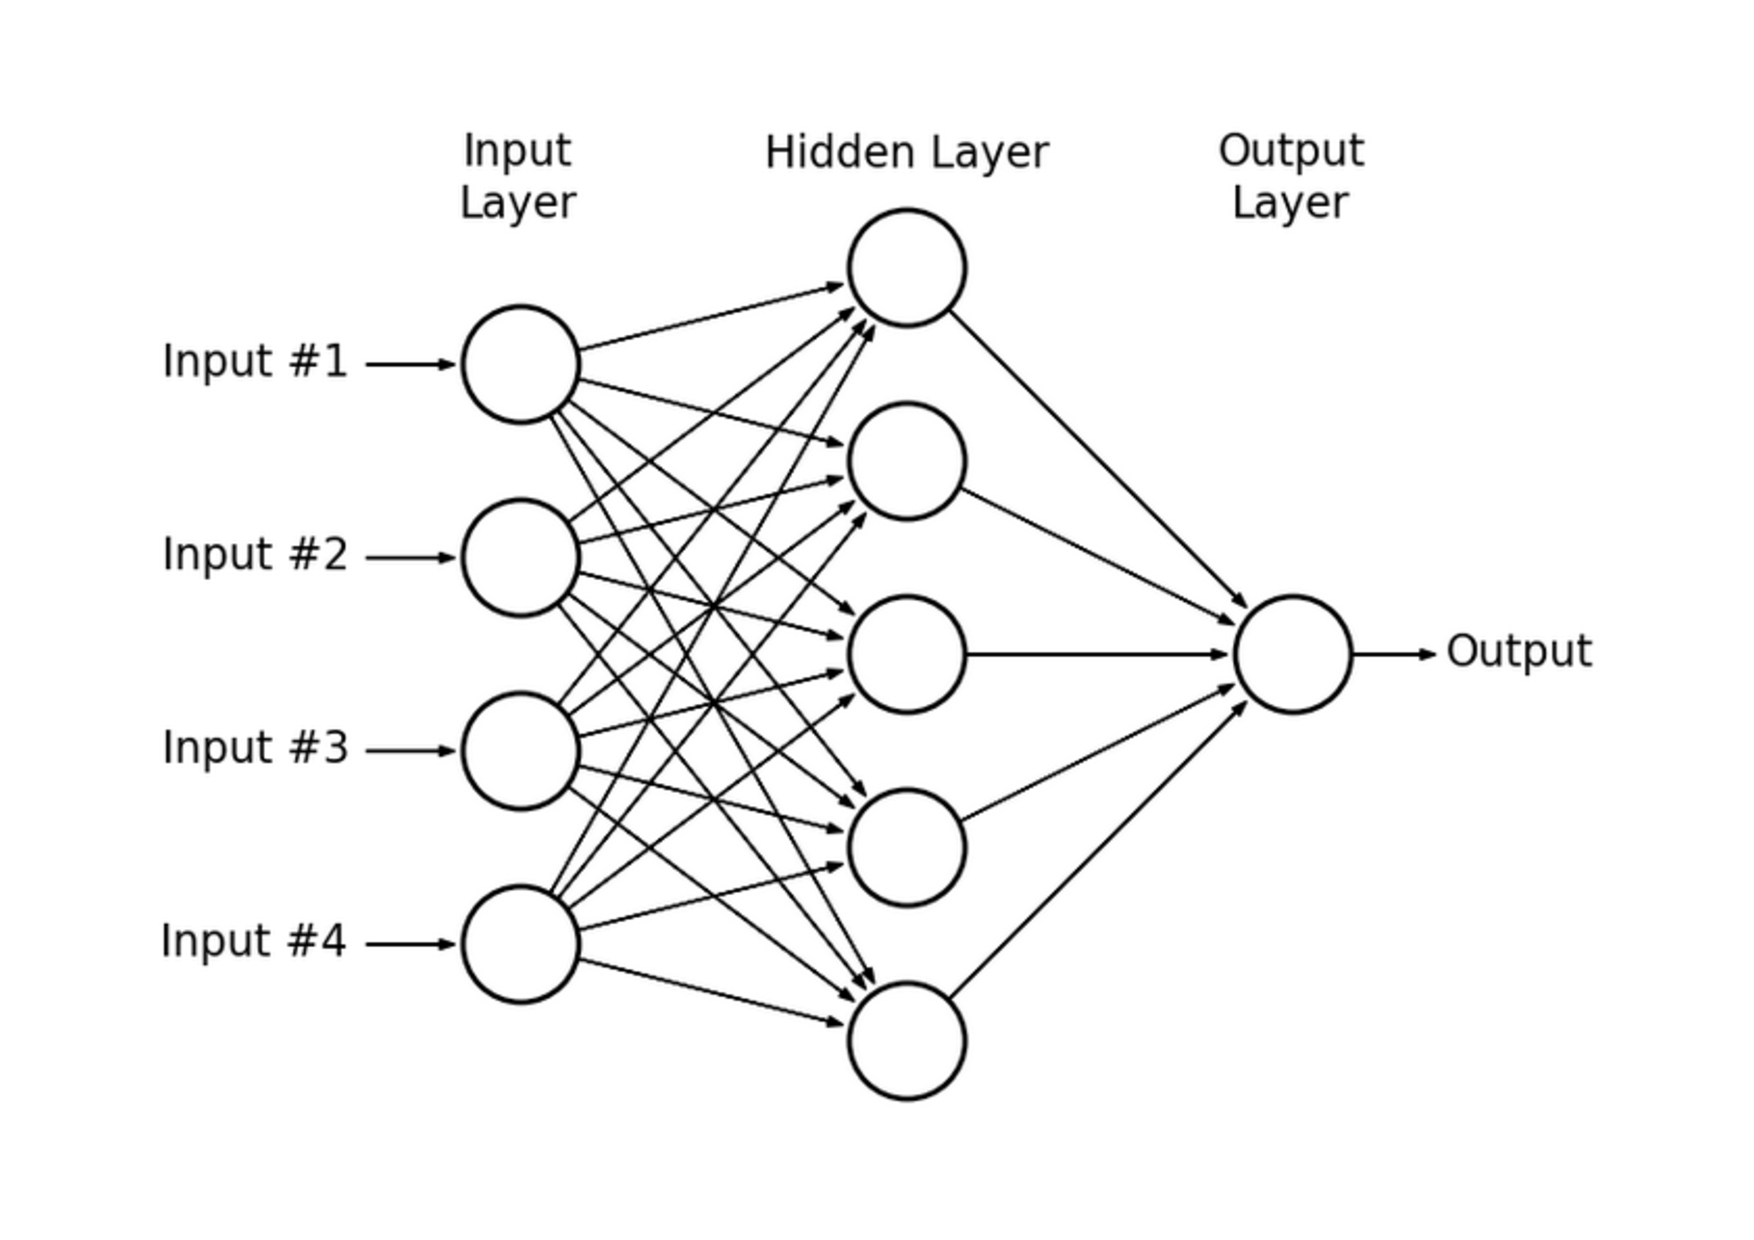
\includegraphics[trim=2cm 2cm 2cm 2cm, clip=true, height=80mm]{Chapter2/FF_Neural_Network.pdf}
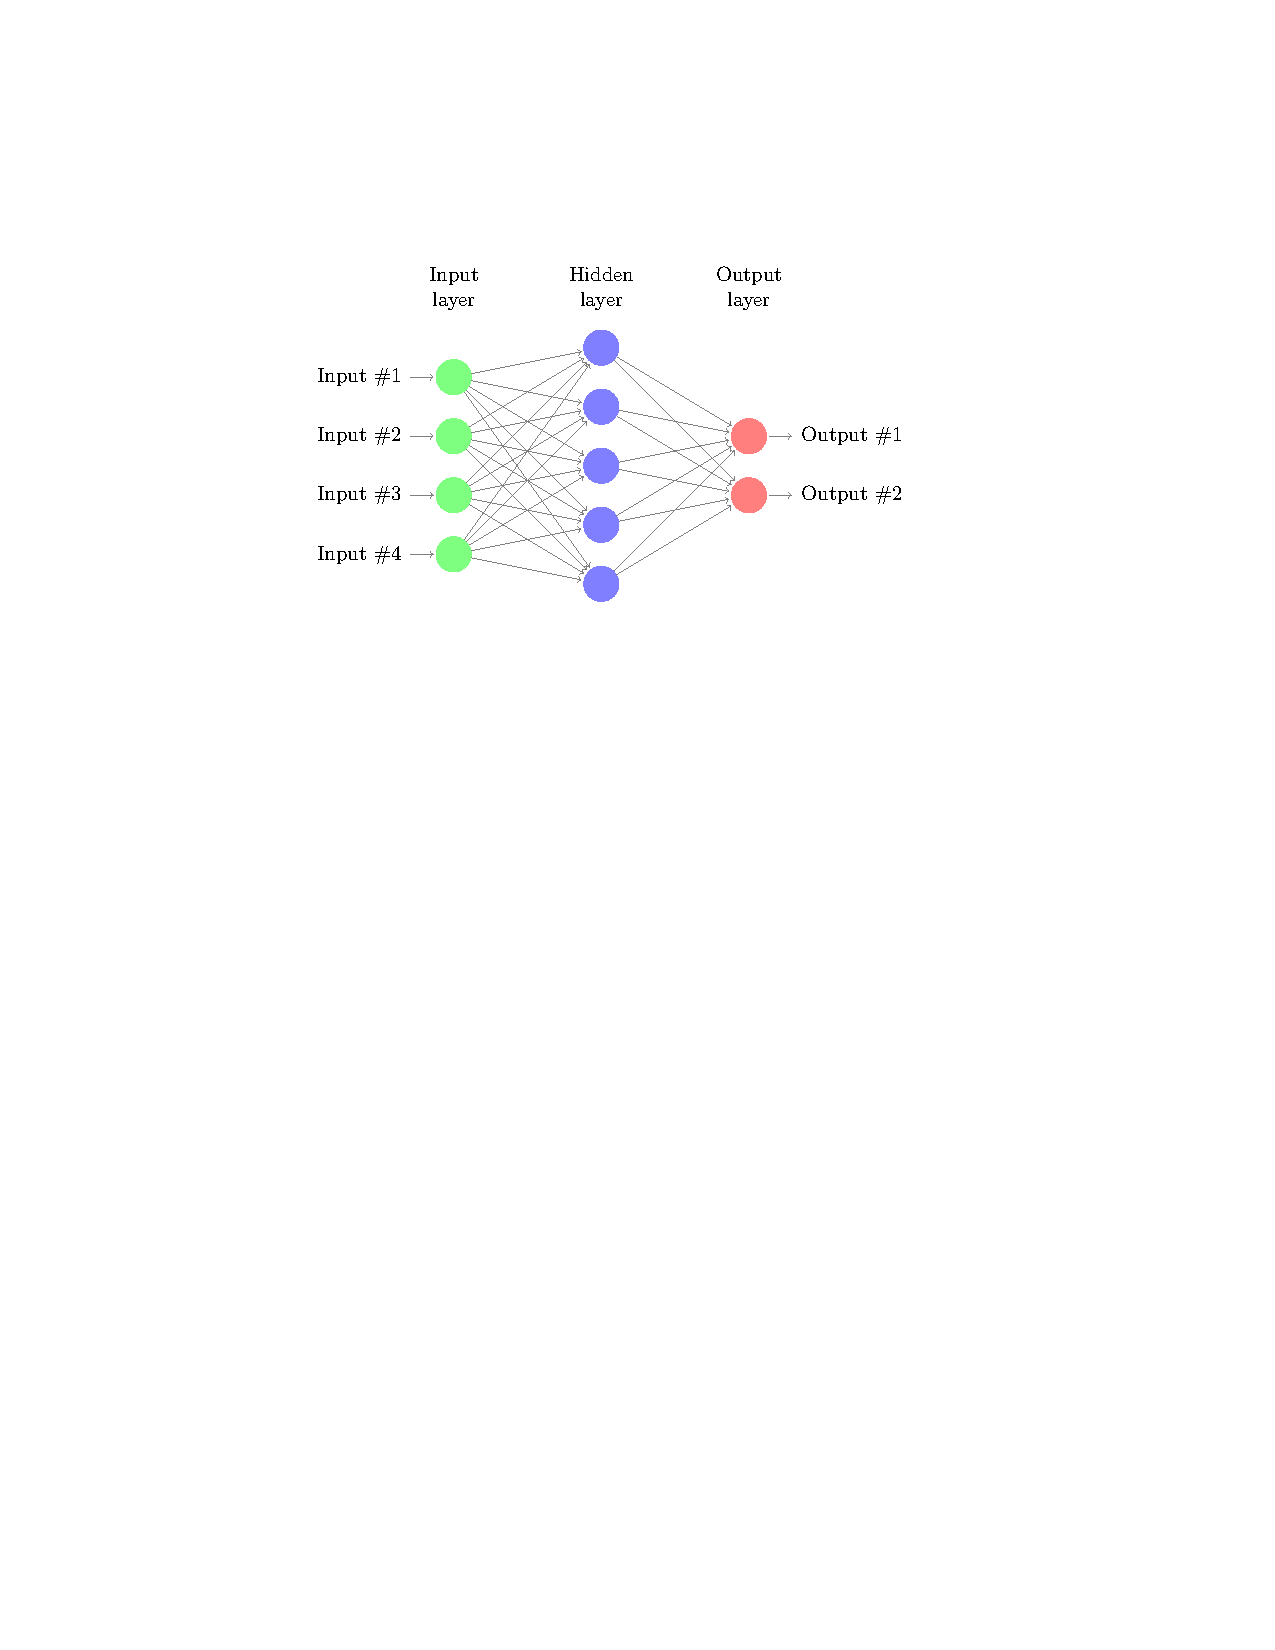
\includegraphics[trim=4cm 17cm 3cm 4cm, clip=true, height=80mm]{Tikz/NN.pdf}
\caption{A 1 layer-feedforward neural network with 4 input nodes, 1 hidden layer with hidden nodes and 2 output node.}
\end{figure}

A feedforward neural network is a standard model in the machine literature for classification problems. It consists of a number of layers composed of simple processing units, also called neurons or nodes, in which each unit in a given layer is connected to a number of units in the previous layers, each connection characterised by a weight encoding the knowledge of the network. Layers in which every unit is only connected to every unit in the previous layer are called fully-connected layers. Each unit represents an activation value generated by passing a linear combination of the values of the incoming connections weighted by their weights to an activation function, such as a Rectified Linear, a Tanh or a Sigmoid function. The information encoded in the data enters at the input layer, gets processed as it passes through the network, layer by layer, until it arrives at the output layer. The choice of the activation function at the output layer is determined by the nature of the data and the assumed distribution of the target variables. For classification problems, the softmax function or, in our case, its log, give the output a probabilistic interpretation. This model can be represented in the form of a network diagram as shown in Figure \ref{Basic_neural_network}.\\

\noindent Training a neural network is done by minimising an error measure of its performance over a training set using gradient-based optimisation routines. The error gradients with respect to the parameters that are needed for the minimisation procedure, can be efficiently evaluated via the standard backpropagation algorithm. To prevent overfitting, a number of regularisation methods are available, including the traditional ones such as L1 and L2 regularisation. Recently a method called dropout \citep{JMLR:v15:srivastava14a} where at every epoch, a percentage of hidden units are randomly deactivated during training has been shown to give better generalisation performance.

\section{Convolutional Neural Networks}

\noindent A CNN is a specialised kind of feedforward neural network where the first few layers of the architecture are so-called convolutional layers. These consist of three stages: a convolution stage, a detection stage and an optional subsampling stage. We will be discussing CNNs in the context of multi-channel images of size $m \times m$, where each pixel value represents an input node. 

\subsection{Convolution}

\begin{figure}
\centering
\label{convolution_operation}
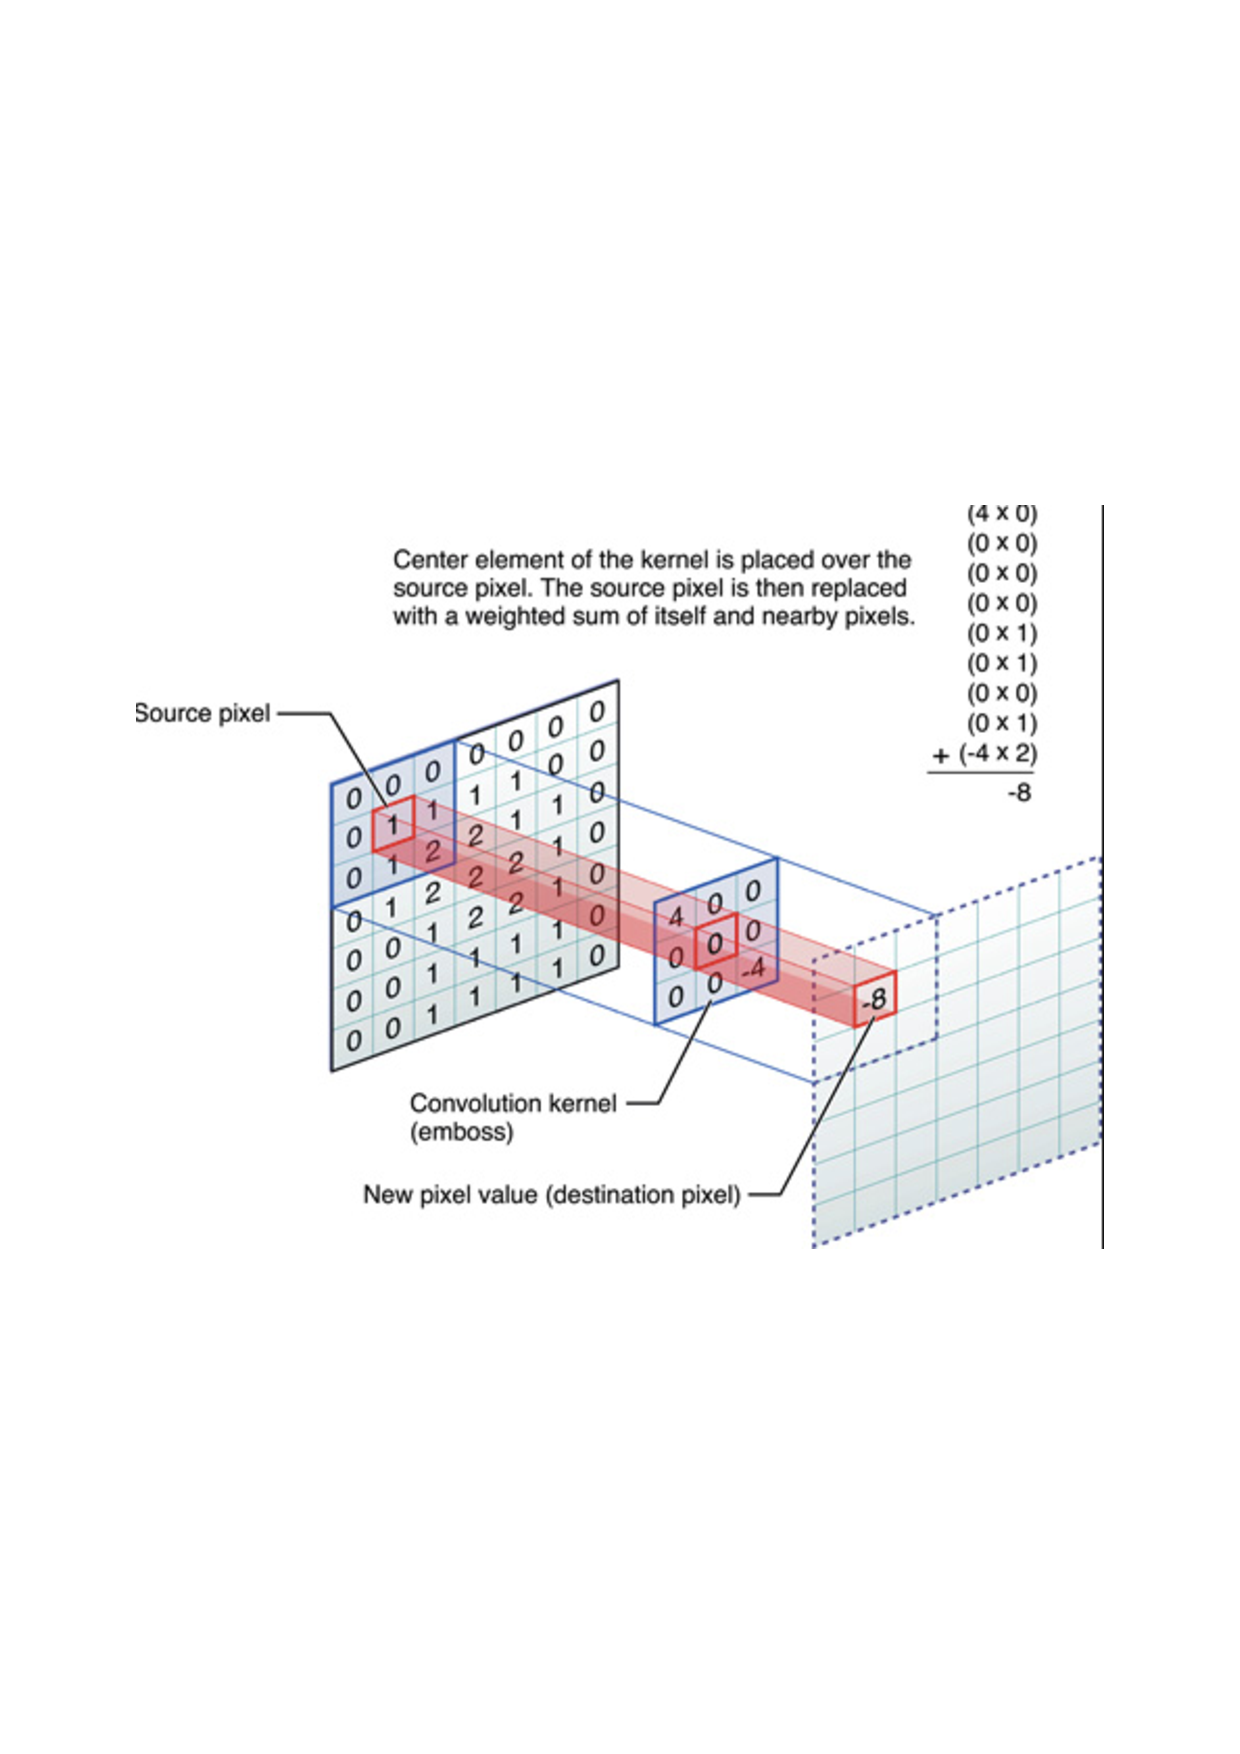
\includegraphics[trim=2cm 7cm 2cm 7cm, clip=true, height=80mm]{Chapter2/convolution.pdf}
\caption{The convolution layer. Illustration of the formation of a feature map.}
\end{figure}

\noindent The convolution stage is responsible for implementing $k$ convolution operations over each channel of the input image. This is accomplished by convolving in parallel each channel with $k$ kernels of size $s \times s$. Unlike fully connected layers, in a convolution, each output node is locally connected to a small square subset of corresponding input nodes determined by the kernel size. Additionally, as the same kernel is applied throughout the image, the convolution operation implies weight sharing, thus greatly reducing the number of trainable parameters. Figure \ref{convolution_operation} illustrates the convolution operation graphically. The set of output nodes resulting from one kernel is called a feature map, which is itself a rectangular arrays of nodes of size $(m - s/2 + 1) \times (m - s/2 + 1)$. Feature maps detect the presence in the input image of a particular feature encoded by the corresponding kernel. Having multiple kernels run through the input layer in parallel produces a set of feature maps. Together, they are responsible for detecting various types of features which might be present in the image. \\

\noindent The benefits of this approach are two folds :

\begin{itemize}
	\item Computational efficiency: the sparse interaction between the hidden nodes and the weight sharing significantly decrease the number of parameters to train.
	\item Translational equivariance: shifting the input results in an equivalent shift in the output. This is a property of the convolution operation.
\end{itemize}

\noindent In the detector stage, every node in the feature map is then passed to an nonlinear activation unit exactly as in a standard neural network. These activation units usually consist of either Rectified Linear units (ReLU), Tanh units, or Sigmoid units.\\

\begin{figure}
\centering
\label{subsampling}
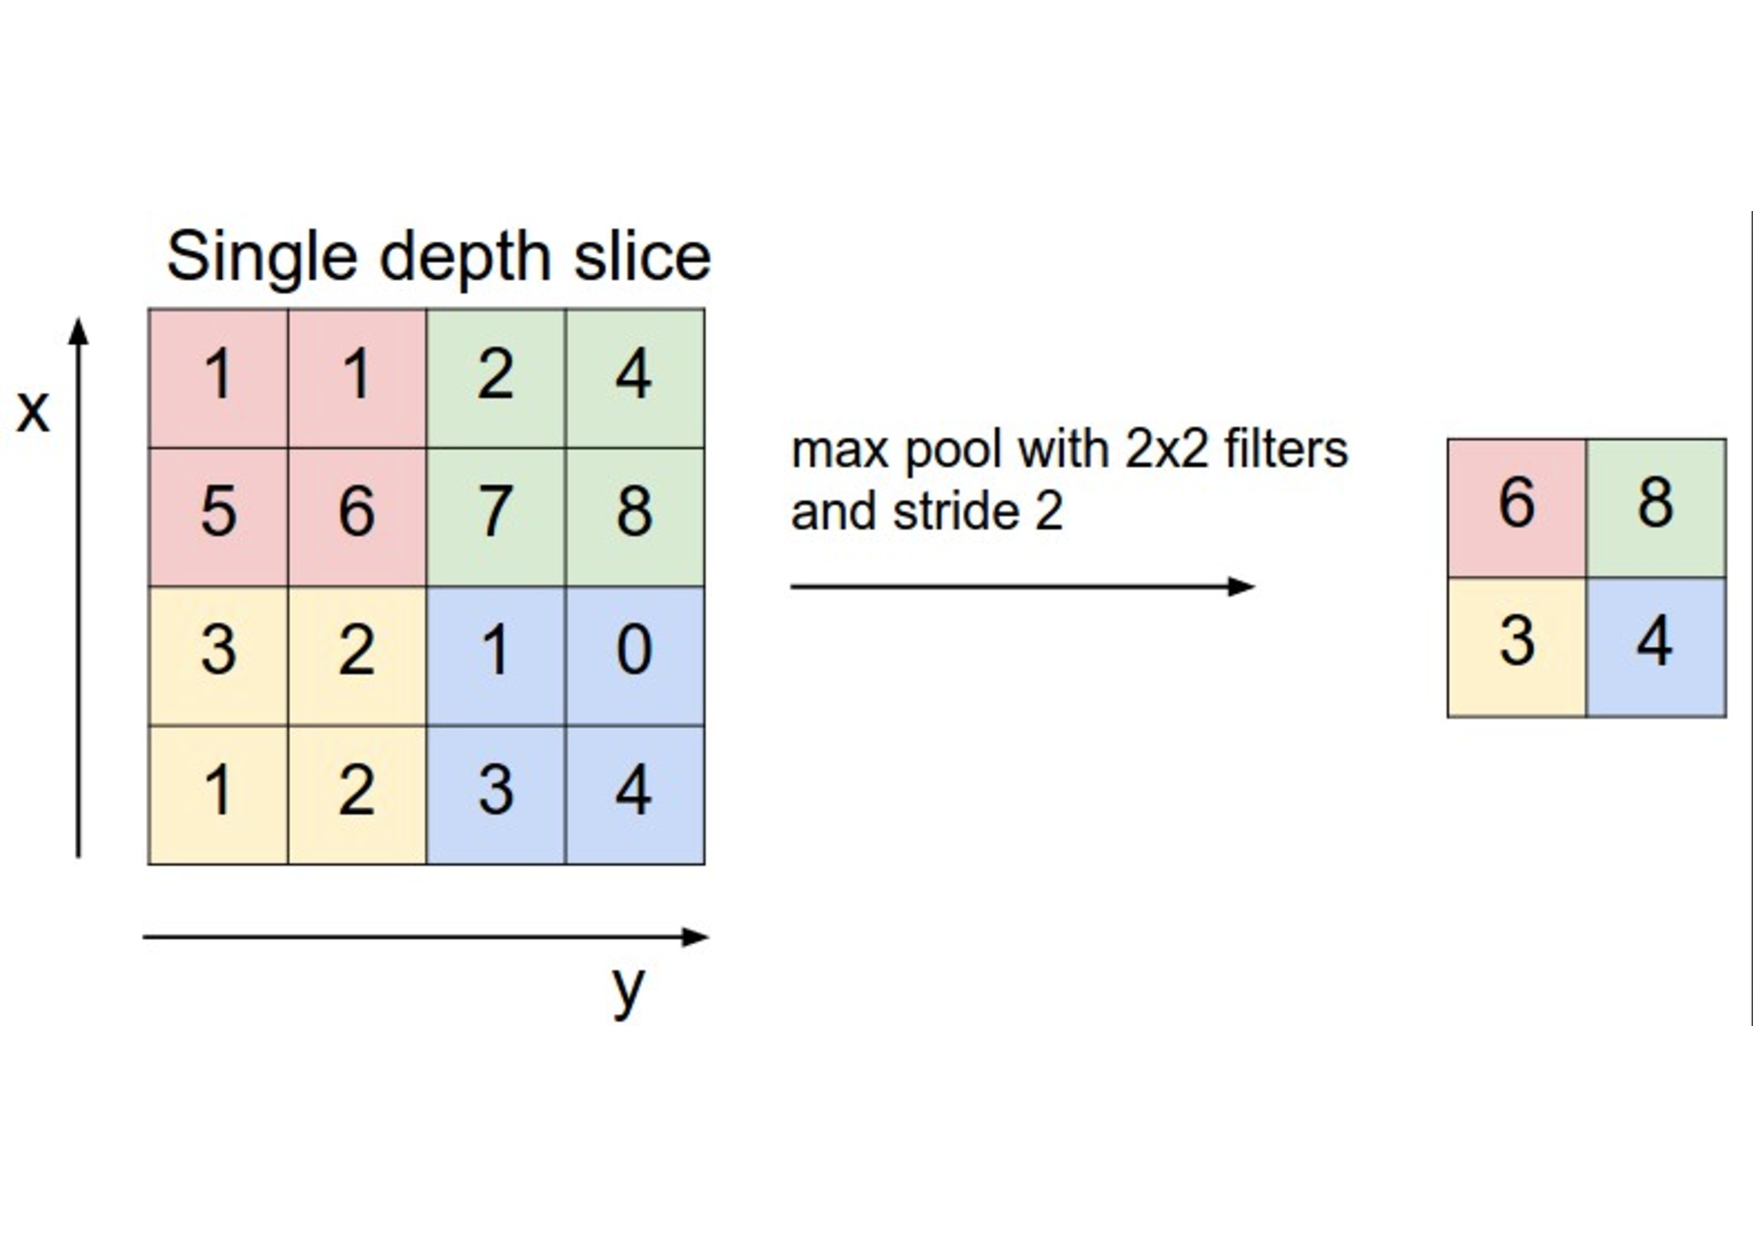
\includegraphics[trim=0cm 0cm 0cm 0cm, clip=true, height=60mm]{Chapter2/pooling.pdf}
\caption{Subsampling in action. Here maxpooling is used to halve the size of an feature map using a $2 \times 2$ filter}
\end{figure}

\noindent Finally in the pooling stage, each feature map is then subsampled by aggregating the node values using a summary statistic over a rectangular neighbourhood of outputs. Two commonly used ones are the max and average pooling operations which report respectively the maximum and average of a set of inputs. Figure \ref{subsampling} shows a diagram of subsampling.\\

\noindent The benefits of subsampling are that it further reduces the number of features by a factor of k for pooling regions spaced k pixels apart, aiding the classification task and improving the computational efficiency of the network. Furthermore subsampling has the added benefit of making the representation become invariant to small translations of the input. Thus translating the input by a small amount results in little to no change in the values of the pooled outputs.\\

\subsection{Typical Architecture}

\noindent A typical convolutional neural network architecture consists of an input layer, a number of convolutional layers, a number of fully connected layers, followed by an output layer. The input layer is an $r \times n \times n$ image, with $r$ being the number of channels and $n$ the image height and width. Each channel is passed through a number convolutional layer in parallel. Then the remaining output nodes from all the resulting feature maps across all channels are "flattened" and passed as input to a number of fully connected layers followed by an output layer. The convolutional layers thus serve as a way to reduce the dimensionality of the image by extracting meaningful local features.








\chapter{Experimental Results}

\section{The Data}

\noindent The aim of this thesis is to implement, and then fine-tune, a CNN to classify voxels of chest computerised tomography (CT) scan as being either in the part of the heart called the atrium or outside of it. The atrium is the entry point of the blood into the heart. It is composed of two chambers: a right one which recovers blood returning to the heart to complete the cardiovascular cycle through the body, and a left one receiving blood coming back from the lungs after being oxygenated.\\

\noindent The data from which the training and testing datasets are generated comprise 27 CT scans. CT scans are 3 dimensional grey scale images, generally of size 480*480*50, generated via computers combining many X-ray images taken from different angles to produce cross-sectional images of specific body parts. They are stored as DICOM files, DICOM standing for Digital Imaging and Communications in Medicine which is a standard for handling, storing, printing, and transmitting information in medical imaging. Each has been segmented by trained radiologists at St Thomas's hospital, the results of which are stored in Nearly Raw Raster Data (NRRD) files, a standard format for storing raster data. These are 3D arrays of the same dimension as their corresponding CT scan with each entry being either a 1 or 0 indicating whether its corresponding voxel belongs in the atrium or not. 

\section{Generating the Datasets: the Tri-Planar Method}

\begin{figure}
\centering
\begin{minipage}{0.45\textwidth}
\centering
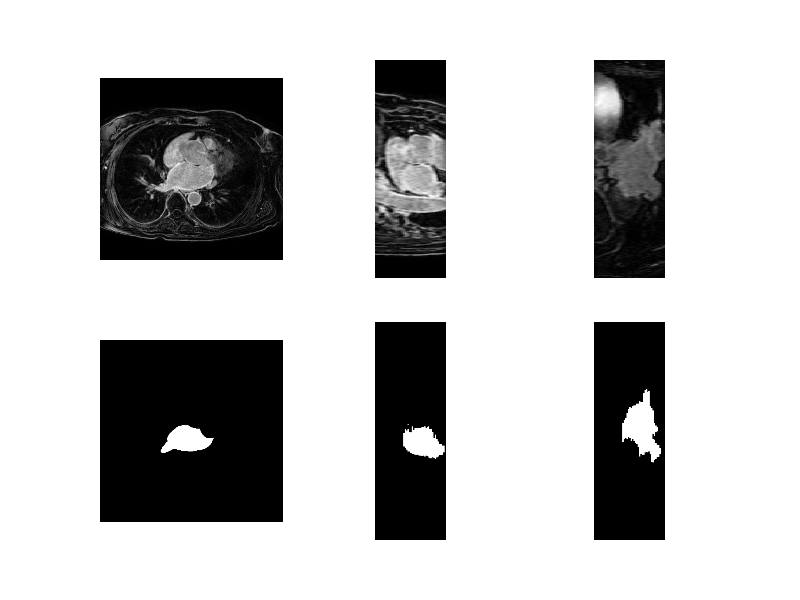
\includegraphics[trim=3cm 1.5cm 3cm 1.5cm, clip=true, height=60mm]{Chapter3/example_slice.png}
\end{minipage}\hfill
\begin{minipage}{0.45\textwidth}
\centering
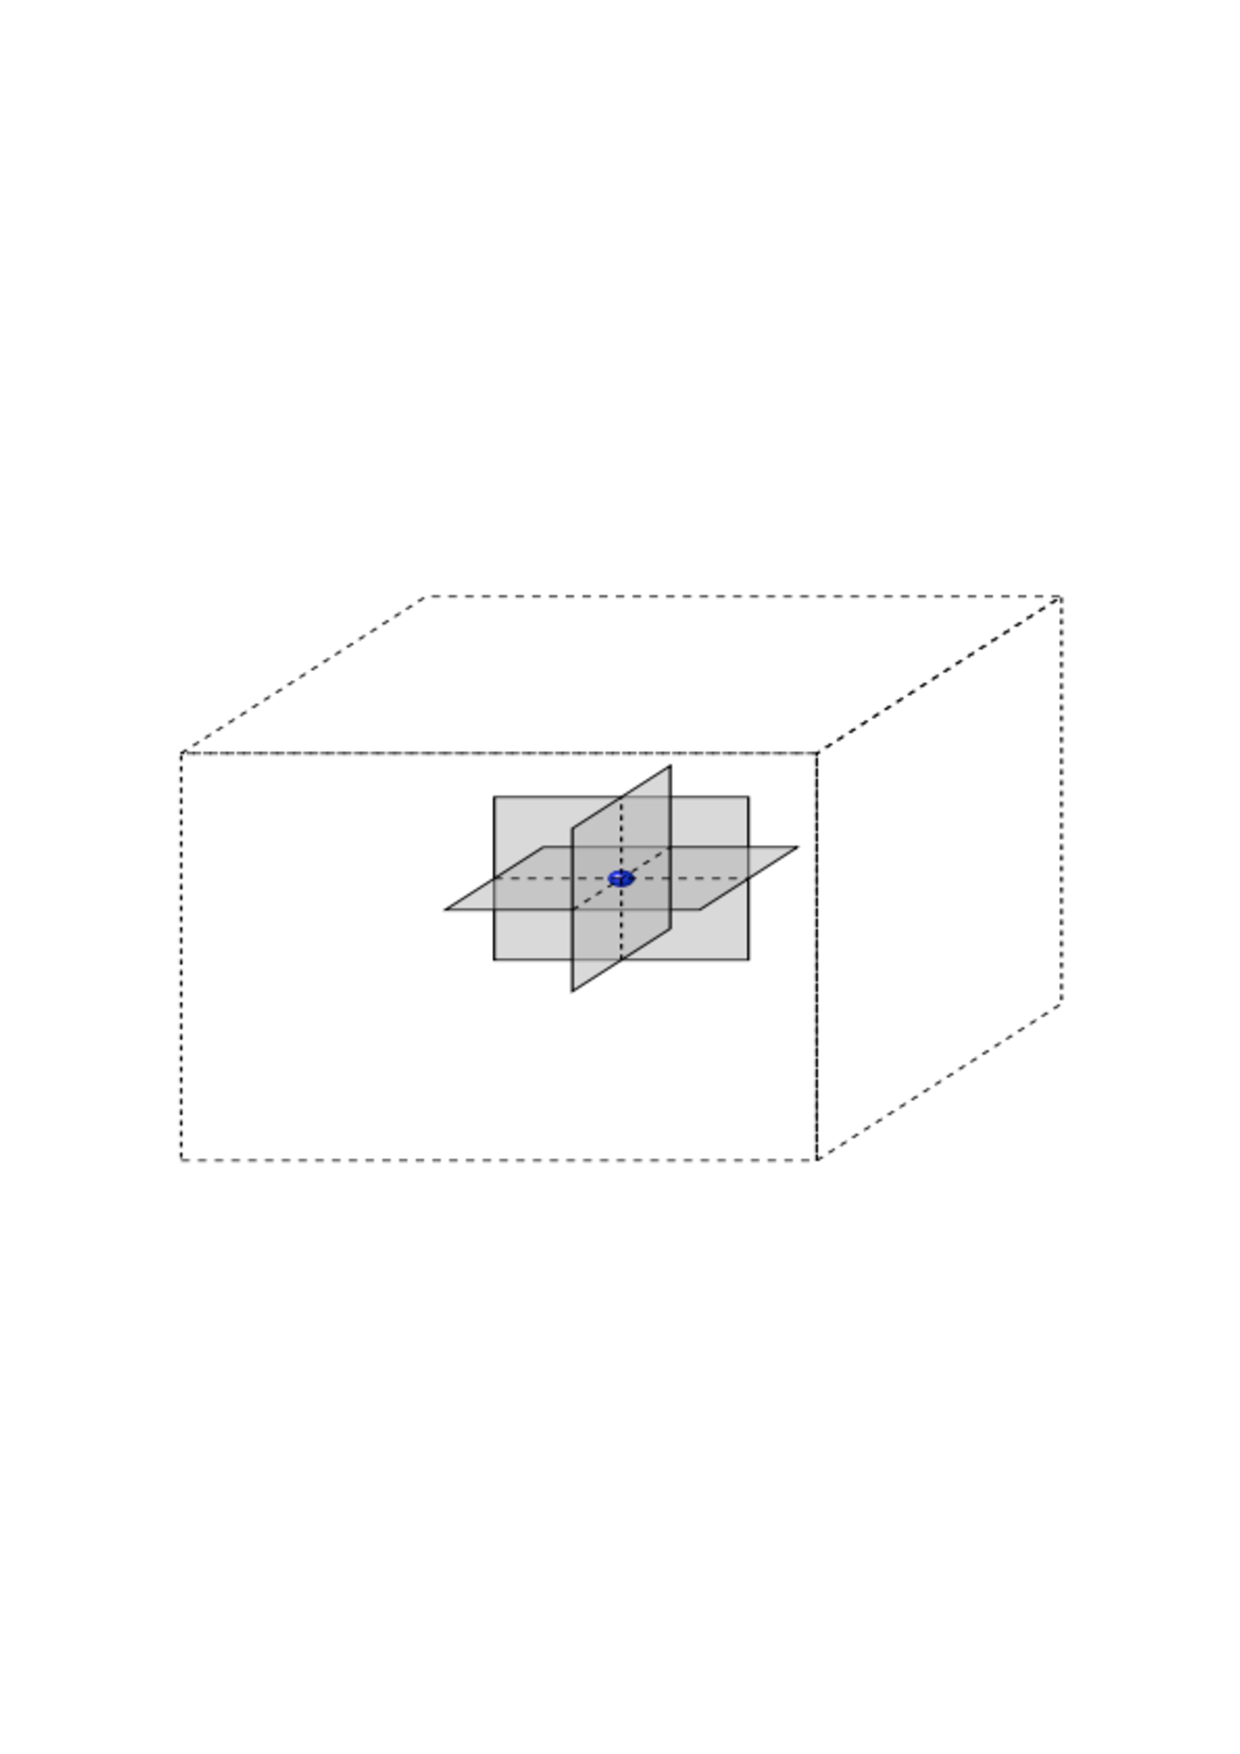
\includegraphics[trim=2cm 8cm 2cm 8cm, clip=true, height=60mm]{Chapter3/triplanar.pdf}
\end{minipage}
\caption{Left: grey scale slices from a CT scan taken in the transversal, saggital and coronal planes. Right: illustration of the triplanar method.}
\label{tri-planar}
\end{figure}

\noindent Classifying the voxels requires building a set of input vectors each containing enough local and global information to allow the neural network to learn effectively. One way of providing 3 dimensional information is to use the tri-planar method. This consists in generating 3 perpendicular square patches of a given dimension in the transversal, saggital and coronal planes centred at the voxel of interest as shown in Figure \ref{tri-planar}. This technique has been found to give competitive results compared to using 3D patches while being much more computationally and memory efficient \citep{knee_cartilage}. In addition, we use a multi-scale approach as in \citep{DBLP:journals/corr/BrebissonM15}, where we add 3 more input channels composed of compressed patches that are originally 5 times larger than the above set of patches, but resized to be of the same size as the first 3 input patches to provide global information about the surroundings of the concerned voxel.\\

\noindent Each patch is fed into a different input channel of the CNN to a total of 6 channels. The outputs of those channels are then feed as inputs to a set of connected layers itself connected to a classifying layer.

\section{Implementation Details}

\subsection{Libraries}

\noindent Our CNNs were implemented using Torch, an open-source library aiming to provide a Matlab-like environment for scientific computing in Lua, along with a number of dependent libraries (nn, cunn, cudnn, fbcunn) which facilitate the training of neural networks on single and multiple GPUs. In addition, we use Python and a number of its libraries to handle all the logistics ranging from generating the datasets to producing plots of segmentation results.

\subsection{Computer facilities}

\noindent The training of the CNNs were conducted alternatively on one of 2 multi-GPU clusters, named montana-nvidia and montana-k80, kindly provided by Prof. Montana. montana-nvidia consists of 24 cores with 129 Gb of memory connected to two NVIDIA Tesla K40m and two Tesla K20Xm while montana-k80 on the other hand has 56 cores with 258 Gb of memory supported by 8 of NVIDIA's Testla K80. 

\section{Model Selection}

\subsection{General Approach for Model Selection}

\noindent In order to find a good set of hyper-parameters for our CNN, we allocate 20 of the 27 CT scans for generating the training set and the remaining 7 for generating the validation set. The training set is composed of 400000 training examples equally divided among the training CT scans, half being in the atrium and the other half outside it. The validation set is composed of 200000 examples equally divided among the testing CT scans. Furthermore at the end of training, each model fully segments a test CT scan to provide performance statistics. From this segmentation are evaluated the model's sensitivity (the percentage of correctly classified atrium voxels), specificity (the percentage of correctly classified non-atrium voxels), and overall classification rate also known as the Dice coefficient, calculated by evaluating the proportion of correctly classified voxels in the segmented image. As 98\% of the CT scan is composed of non-atrium voxels, the Dice coefficient is overwhelmingly influenced by the specificity. We will conduct our model selection by selectively choosing hyper-parameters that optimise the Dice coefficient while having a reasonable sensitivity above 0.8.\\

\noindent Additionally, mask images are generated from 3 transversal slices in the segmented CT scan. The masks are formed by overlaying the grey scale CT scan image with colours representing the error status of the classification of a given voxel. They provide a visual representation of the performance of the models. The colour codes are:

\begin{itemize}
	\item Green: correctly classified atrium voxel.
	\item Blue: correctly classified non-atrium voxel.
	\item Red: incorrectly classified atrium voxel.
	\item Pink: incorrectly classified non-atrium voxel.
\end{itemize}

\noindent We start off our model selection with a CNN comprised of an input layer with 6 channels of patches of size 32*32, 2 convolutional layers with 32 and 64 feature maps respectively and a max pooling filter of size $2 \times 2$, 2 fully connected layers with 1000 and 500 hidden units each respectively, and a logsoftmax output layer giving the log probabilities of the voxel belonging to either classes. The training parameters are composed of a learning rate of 0.01, a momentum rate set to 0, and a mini-batch size set to 6000 examples. In addition, the negative log likelihood criterion provides the error measure during training. We will be varying in turn the following hyper-parameters while at each stage keeping the others constant.\\

\begin{itemize}
	\item the number of convolutional layers.
	\item the number of connected layers.
	\item the number of feature maps in the chosen number of convolutional layers.
	\item the number of hidden units in the chosen number of connected layers.
	\item the learning rate.
	\item the momentum.
	\item the type of activation function (ReLU, Tanh or Sigmoid).
\end{itemize}

\subsection{Varying the Number of Convolutional Layers}

\noindent To select the number of convolutional layers, we train 4 CNNs with architectures starting with the following convolutional layers:

\begin{itemize}
	\item Input (6*32*32) => Conv layer (32*28*28) => 2*2 MaxPooling filter (32*14*14) 
	\item Input (6*32*32) => Conv layer (32*28*28) => 2*2 MaxPooling filter (32*14*14) => Conv layer (64*10*10) => 2*2 MaxPooling filter (64*5*5)
	\item Input (6*32*32) => Conv layer (32*28*28) => Conv layer (32*24*24) => 2*2 MaxPooling filter (32*12*12) => Conv layer (64*8*8) => 2*2 MaxPooling filter (64*4*4)
	\item Input (6*32*32) => Conv layer (32*28*28) => Conv layer (32*24*24) => 2*2 MaxPooling filter (32*12*12) => Conv layer (64*8*8) => Conv layer (64*4*4) => 2*2 MaxPooling filter (64*2*2)
\end{itemize}

\noindent The values in parentheses indicate the number and dimensions of the feature maps at each layer. The following table gives the results for each of these architectures trained over 100 epochs.\\

{
\centering
\begin{tabular}{cccccc}
\rowcolor[HTML]{C0C0C0} 
        \# Conv Layers & Sensitivity & Specificity & Test Dice Coefficient \\ \hline
1  &      0.913       & 0.970       & 0.969                                                        \\ 
2  &      0.734       & 0.989       & 0.984                                                        \\ 
3  &      0.762       & 0.987       & 0.983                                                        \\ 
4  &      0.881       & 0.973       & 0.972                                                       
\end{tabular}\\
\vspace{0.5cm}
}

\begin{figure}
\centering
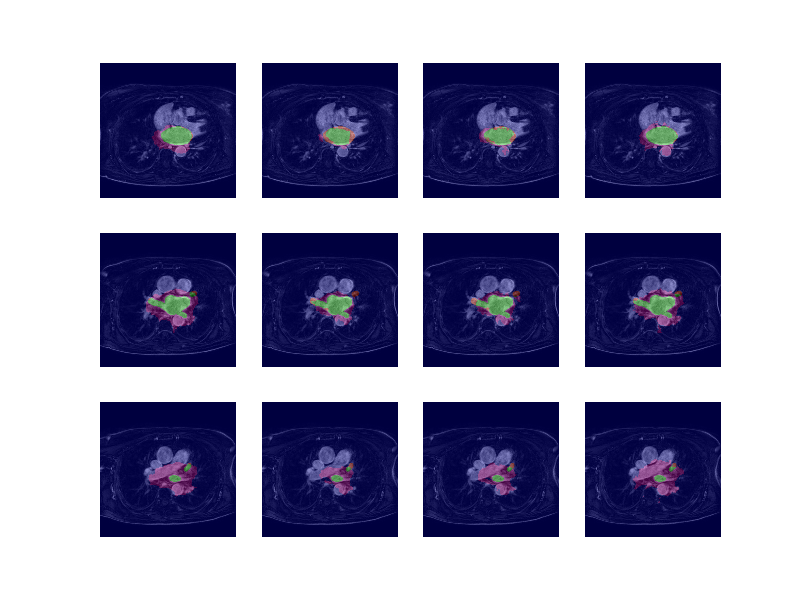
\includegraphics[trim=2.5cm 1.5cm 2cm 1.5cm, clip=true, height=80mm, width=150mm]{Chapter3/mask_results_varying_number_of_convolutional_layers.png}
\caption{Masks for varying number of convolutional layers. Each row displays the same mask generated by CNNs with from left to right, 1, 2, 3 and 4 convolutional layers.}
\label{mask_varying_conv_layers}
\end{figure}

\noindent The architecture with the best test Dice coefficient is the one with 2 convolutional layers, closely followed by the one with 3 convolutional layers, with Dice coefficients of 0.984 and 0.983 respectively. These two architectures give low sensitivities of 0.734 and 0.762. The architectures with 1 and 4 convolutional layers yield significantly lower Dice coefficients of 0.969 and 0.972 respectively, despite a much greater sensitivity of 0.913 and 0.881. \\

\noindent Figure \ref{mask_varying_conv_layers} shows the masks from all 4 models generated after training. The first and fourth columns correspond to segmentations by the architectures with 1 and 4 convolutional layers respectively. These show much larger pink patches, corresponding to higher rates of false positives than the other two columns but with smaller red regions corresponding to lower rates of false negatives, corroborating the story told by the sensitivity and specificity in the table above. There is not much difference between the masks of the second and third layers.\\

\noindent We choose the architecture with the highest Dice coefficient at this stage and thus select an architecture with 2 convolutional layers. 

\subsection{Varying the Number of Connected Layers}

\noindent Having settled on an architecture with 2 convolutional layers, we now train 3 CNNs with 1, 2, and 3 fully connected layers each starting with 1000 hidden units and halving the number of hidden units for each additional layer. Hence the CNN with 3 fully connected layers has 1000, 500, and 250 hidden units in each of its successive layers. The results are shown in the following table.\\

{
\centering
\begin{tabular}{cccccc}
\rowcolor[HTML]{C0C0C0} 
             \# Connected Layers & Sensitivity & Specificity & Test Dice Coefficient \\ \hline
1  & 0.887       & 0.972       & 0.971                                                        \\ 
2  & 0.856       & 0.974       & 0.972                                                        \\ 
3  & 0.915       & 0.967       & 0.966                                                       
\end{tabular}\\
\vspace{0.5cm}
}

\begin{figure}
\centering
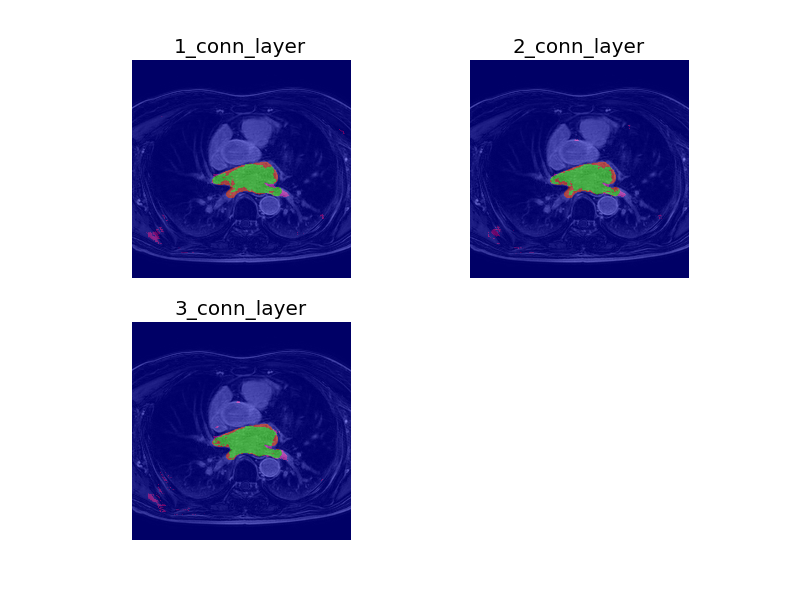
\includegraphics[trim=2.5cm 1.5cm 2cm 1.5cm, clip=true, height=80mm, width=150mm]{Chapter3/mask_results_varying_number_of_connected_layers.png}
\caption{Masks for varying number of connected layers. Each row displays the same mask generated by CNNs with from left to right, 1, 2, and 3 connected layers.}
\label{mask_varying_connected_layers}
\end{figure}

\noindent All three architectures have similar performances on the test CT scan. The architectures with 1 and 2 connected layers in particular have the highest Dice coefficients of the three with marginally different specificities of 0.972 and 0.974 respectively. The discrepancies between their sensitivities are somewhat more pronounced at 0.887 and 0.856 respectively. Figure \ref{mask_varying_connected_layers} similarly shows very little differences in the colour profile of the masks for all three architectures. Thus it seems that adding extra connected layers doesn't significantly increase the performance of the classifier and hence we opt for having 1 fully connected layer in our final architecture.

\subsection{Varying the Number of Feature Maps}

\noindent We now focus on finding the right number of feature maps for the convolutional layers. In order to keep the computation comparable between the 2 layers, we set the number of feature maps in the second layer to be twice that of the first layer. We try configurations with the first layer having 16, 32, and 64 feature maps. The summary of the results are shown below.\\

{
\centering
\begin{tabular}{cccccc}
\rowcolor[HTML]{C0C0C0} 
          Feature Maps & Sensitivity & Specificity & Test Dice Coefficient \\ \hline
 16  & 0.919       & 0.967       & 0.966                                                        \\ 
 32  & 0.894       & 0.972       & 0.970                                                        \\ 
 64  & 0.904       & 0.971       & 0.970                                                        
\end{tabular}\\
\vspace{0.5cm}
}

\begin{figure}
\centering
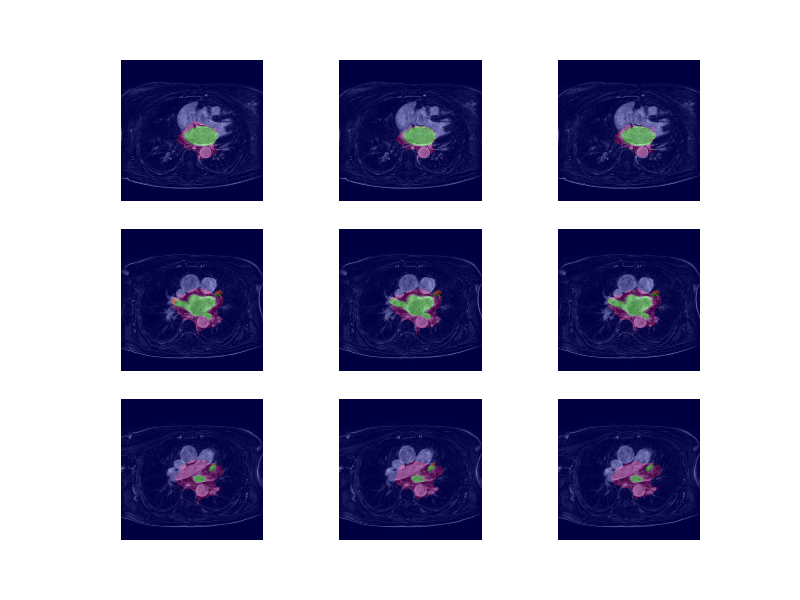
\includegraphics[trim=2.5cm 1.5cm 2cm 1.5cm, clip=true, height=80mm, width=150mm]{Chapter3/mask_results_varying_number_of_feature_maps.png}
\caption{Masks for varying number of feature maps. Each row displays the same mask generated by CNNs with from left to right, 16, 32, and 64 feature maps in their first convolutional layers.}
\label{mask_varying_feature_maps}
\end{figure}

\noindent Again the differences between the performance of all three architectures are minimal. The architectures with a first layer having 32 and 64 feature maps have the highest Dice coefficient both at 0.970 and very similar sensitivities around 0.9. The architecture with 16 feature maps yields a slightly lower specificity of 0.967 but a higher sensitivity of 0.919 with an overall lower Dice coefficient of 0.966. Figure \ref{mask_varying_feature_maps} show slight differences in the first row of images, with a larger pink region for the 16 feature map architecture. \\

\noindent As the highest test Dice coefficient belongs to the architecture with 32 and 64 feature maps, we opt for the simpler model and have 32 feature maps in the first layer of our final architecture.

\subsection{Varying the Number of Hidden Units}

\noindent We now vary the number of hidden units in the connected layer, trying 100, 200, 500, 1000 hidden units. \\

{
\centering
\begin{tabular}{cccccc}
\rowcolor[HTML]{C0C0C0} 
                 Hidden Units & Sensitivity & Specificity & Test Dice Coefficient \\ \hline
100   & 0.879       & 0.972       & 0.97                                                         \\ 
200   & 0.878       & 0.971       & 0.97                                                         \\ 
500   & 0.894       & 0.97        & 0.968                                                        \\ 
1000  & 0.892       & 0.972       & 0.97                                                        
\end{tabular}\\
\vspace{0.5cm}
}

\begin{figure}
\centering
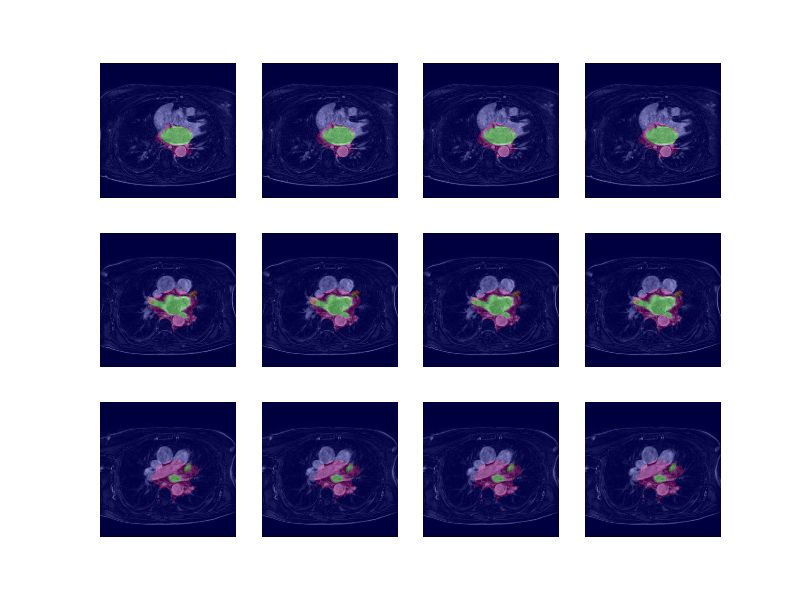
\includegraphics[trim=2.5cm 1.5cm 2cm 1.5cm, clip=true, height=80mm, width=150mm]{Chapter3/mask_results_varying_number_of_hidden_units.png}
\caption{Masks for varying number of hidden units. Each row displays the same mask generated by CNNs with from left to right, 100, 200, 500, and 1000 hidden units in the connected layer.}
\label{mask_varying_hidden_units}
\end{figure}

\noindent The results across all 4 models are very similar. Indeed the architectures with 100, 200, and 1000 hidden units yield test Dice coefficients of 0.97 and the one with 500 hidden units has a slightly lower one at 0.968. Their sensitivities are also very close, being at 0.879, 0.878, 0.894 and 0.892 respectively. Figure \ref{mask_varying_hidden_units} shows mask results with little differences between models as well. \\

\noindent We choose the simpler model of the 4 and elect to have 100 hidden units in our final architecture.\\

\subsection{Varying the Learning Rate}

\noindent Having established our final architecture, we now turn our attention to choosing the learning rate. We try learning rates of 0.01, 0.05, 0.1, 0.5 and 1. The results are shown in the following table, although we omitted the results for a learning rate of 1 as the CNN didn't train.\\

{
\centering
\begin{tabular}{cccccc}
\rowcolor[HTML]{C0C0C0} 
Learning Rate &  Sensitivity & Specificity & Test Dice Coefficient \\ \hline
\rowcolor[HTML]{FFFFFF} 
 0.01                                                 & 0.885       & 0.971       & 0.97                                                         \\
\rowcolor[HTML]{FFFFFF} 
 0.05                                                 & 0.915       & 0.977       & 0.976                                                        \\ 
\rowcolor[HTML]{FFFFFF} 
 0.1                                                  & 0.916       & 0.98        & 0.978                                                        \\
\rowcolor[HTML]{FFFFFF} 
 0.5                                                  & 0.932       & 0.982       & 0.981                                                       
\end{tabular}\\
\vspace{0.5cm}
}

\begin{figure}
\centering
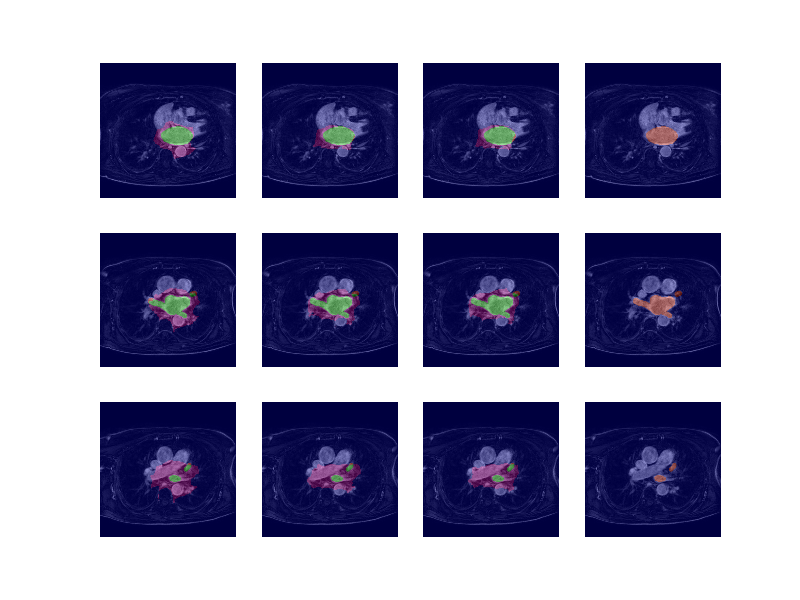
\includegraphics[trim=2.5cm 1.5cm 2cm 1.5cm, clip=true, height=80mm, width=150mm]{Chapter3/mask_results_varying_learning_rate.png}
\caption{Mask for varying learning rate. Each row displays the same mask generated by CNNs with from left to right, learning rates of 0.01, 0.05, 0.1 and 0.5.}
\label{mask_results_learnin_rate}
\end{figure}

\noindent The table shows improved results as the learning rate increases. The test Dice coefficient jumps substantially from 0.97 for a learning rate of 0.01 to 0.981 for a learning rate of 0.5. So does the sensitivity from 0.885 for a learning rate of 0.01 to 0.932 for a learning rate of 0.5. The masks shown in Figure \ref{mask_results_learnin_rate} reflect this improvement in accuracy with a substantial decrease of the size of the pink regions as the learning rate increases. The mark difference in performance illustrate the importance of setting an appropriate learning rate.\\

\noindent We thus choose a learning rate of 0.5 to train our selected architecture.

\subsection{Varying the Momentum}

\noindent We now train our CNN with a variety of momentums. We train with momentums set to 0, 0.05, 0.01, 0.5 and 1. The results are shown in the following table, albeit without those for a momentum set to 1 as the network didn't train.\\

{
\centering
\begin{tabular}{cccccc}
\rowcolor[HTML]{C0C0C0} 
Momentum & Sensitivity & Specificity & Test Dice Coefficient \\ \hline
\rowcolor[HTML]{FFFFFF} 
0        & 0.906       & 0.982       & 0.981                                                        \\ 
\rowcolor[HTML]{FFFFFF} 
0.05     & 0.916       & 0.98       & 0.979                                                        \\ 
\rowcolor[HTML]{FFFFFF} 
0.1      & 0.9         & 0.984         & 0.982                                                        \\
\rowcolor[HTML]{FFFFFF} 
0.5      & 0.83        & 0.988        & 0.985                                                       
\end{tabular}\\
\vspace{0.5cm}
}

\begin{figure}
\centering
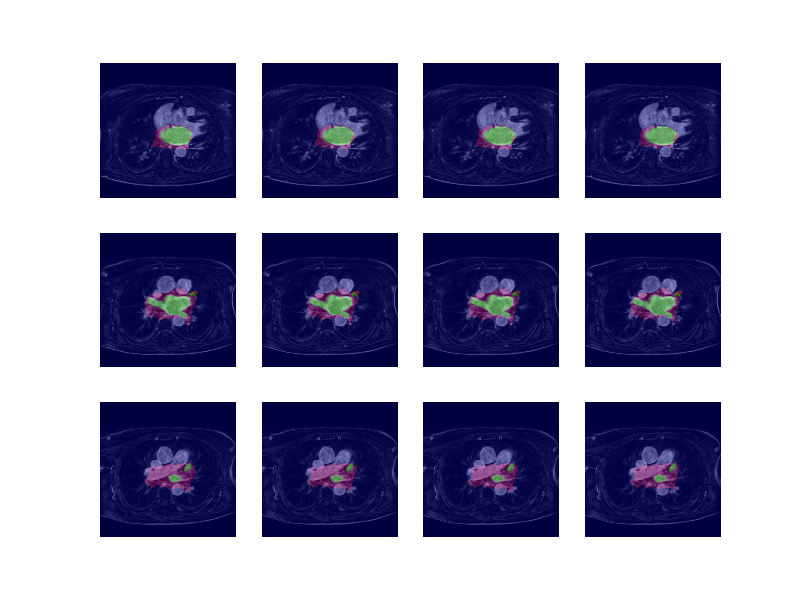
\includegraphics[trim=2.5cm 1.5cm 2cm 1.5cm, clip=true, height=80mm, width=150mm]{Chapter3/mask_results_varying_momentum.png}
\caption{Masks for varying momentum. Each row displays the same mask generated by CNNs with from left to right, momentum set to 0, 0.05, 0.1 and 0.5.}
\label{mask_results_momentum}
\end{figure}

\noindent The momentum yielding the best test Dice coefficient is the one set at 0.05 with an accuracy of 0.985, despite having the lowest sensitivity of 0.83. The test results for the other networks are fairly similar with test Dice coefficients of 0.981, 0.979 and 0.982, and sensitivities of 0.906, 0.916 and 0.9 for those with momentums of 0, 0.05 and 0.1 respectively. Here there is a tradeoff between the overall accuracy and the sensitivity. Figure \ref{mask_results_momentum} shows the slight improvement of overall accuracy.\\

\noindent As the one with the highest Dice coefficient, we set our momentum to 0.5.

\subsection{Varying the Activation Function}

\noindent As the last step towards choosing our final architecture, we experiment with the 3 main types of possible activation function: ReLU, Tanh, Sigmoid. The results are shown in the table below\\

{
\centering
\begin{tabular}{cccccc}
\rowcolor[HTML]{C0C0C0} 
Activation Function & Sensitivity & Specificity & Test Dice Coefficient \\ \hline
\rowcolor[HTML]{FFFFFF} 
ReLU                                                          & 0.87        & 0.986       & 0.984                                                        \\
\rowcolor[HTML]{FFFFFF} 
Tanh                                                          & 0.934       & 0.98        & 0.979                                                        \\
\rowcolor[HTML]{FFFFFF} 
Sigmoid                                                       & 0.941       & 0.968       & 0.967                                                       
\end{tabular}\\
\vspace{0.5cm}
}

\begin{figure}
\centering
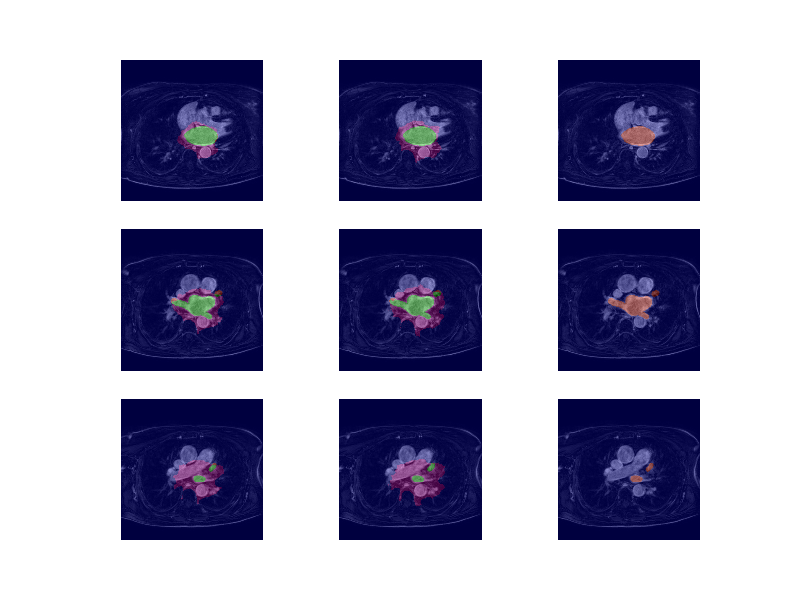
\includegraphics[trim=2.5cm 1.5cm 2cm 1.5cm, clip=true, height=80mm, width=150mm]{Chapter3/mask_results_varying_activation_function.png}
\caption{Masks for varying activation function. Each row displays the same mask generated by CNNs with from left to right, ReLU, Tanh and Sigmoid activation functions.}
\label{mask_varying_activation_function}
\end{figure}

\noindent As could be expected, the architecture with ReLU activation functions performed better overall with the highest Dice coefficient of the 3 at 0.984, followed by the ones with Tanh and Sigmoid activation functions at 0.979 and 0.967. However its sensitivity is the lowest of the three at 0.87, with the ones for the Tanh and Sigmoid at 0.934 and 0.941 respectively. The mask results shown in Figure \ref{mask_varying_activation_function} are very similar across all three models. \\

\noindent Unsurprisingly, we opt for an architecture with ReLU activation functions.

\newpage

\section{Sampling Method}

\noindent We now look at a possible improvement of the sampling method used for obtaining the training dataset. As most of the classification errors lie in the border regions of the atrium, one obvious avenue of improvement is to increase the proportion of examples in that region. To that end, we consider a rectangular box containing the atrium, which we call the atrium box.\\

\begin{figure}
\centering
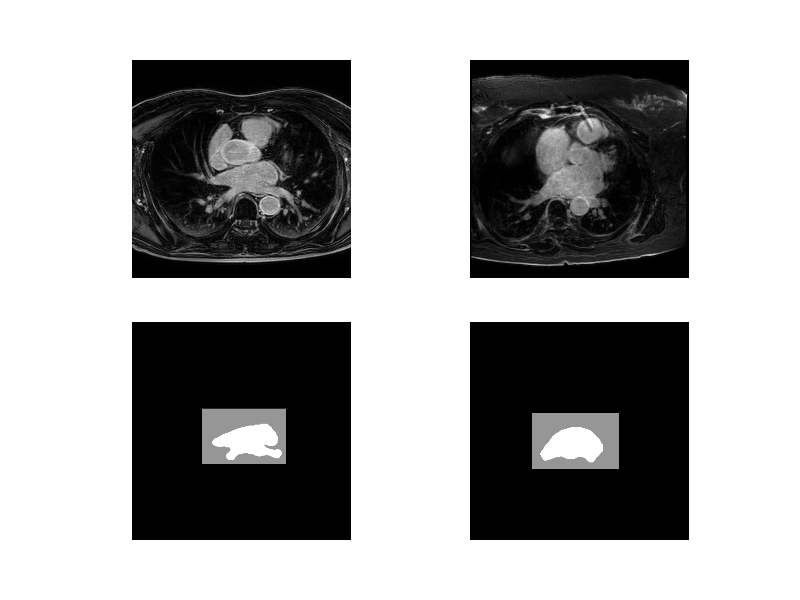
\includegraphics[trim=2.5cm 1.5cm 2cm 1.5cm, clip=true, height=80mm, width=150mm]{Chapter3/sampling_example.png}
\caption{Images illustrating the atrium box. The top row contains transversal slices of 2 different CT scans and the bottom row, their labelling with, in black, non-atrium voxels outside the atrium box, in grey, non-atrium voxels inside the atrium box, and in white, atrium voxels.}
\label{sampling_example}
\end{figure}

\noindent Such a box is constructed by going through all the coordinates of the voxels in the atrium, pick the minimum and maximum coordinate values in each of the coordinate planes, and possibly add some padding. Figure \ref{sampling_example} shows 2 transversal slices of different CT scans with their labels, where the non-atrium voxels inside the atrium box are in grey. A simple modification of our sampling procedure would be to sample half of the non-atrium voxels inside the box and half outside it.  \\

\noindent We train our selected CNN using datasets generated from 3 sampling procedures: using no atrium box, using a small atrium box constructed by the procedure above with a padding of 5 pixels in the transversal plane and of 1 pixel in the remaining coordinate direction, and finally a large atrium box with a padding of 30 pixels in the transversal plane and of 5 pixels in the remaining coordinate direction. The test results are shown in the table below.\\

{
\centering
\begin{tabular}{cccccc}
Sampling Type & Sensitivity & Specificity & Test Dice Coefficient \\ \hline
No Atrium Box                                              & 0.881       & 0.986       & 0.984                                                        \\
Small Atrium Box                                           & 0.838       & 0.994       & 0.991                                                        \\
Large Atrium Box                                           & 0.871       & 0.989       & 0.987                                                       
\end{tabular}\\
\vspace{0.5cm}
}

\begin{figure}
\centering
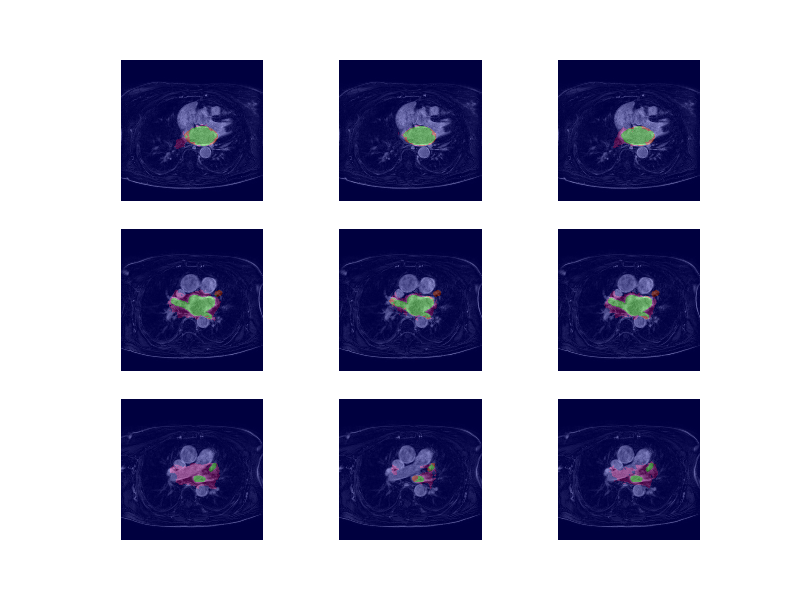
\includegraphics[trim=2.5cm 1.5cm 2cm 1.5cm, clip=true, height=80mm, width=150mm]{Chapter3/mask_results_varying_training_dataset.png}
\caption{Masks for varying training dataset. Each row displays the same mask generated by CNNs with from left to right, using training datasets generated with no atrium box, a small atrium box, and a large box}
\label{training_dataset}
\end{figure}

\noindent Sampling using the small atrium box yield a substantial improvement of the Dice coefficient, raising it to 0.991 against 0.984 with a large atrium box and 0.984 with no atrium box. However the sensitivity is negatively affected, dropping from 0.881 by sampling with no atrium box, to 0.871 with a large one and more still to 0.838 with a small one. Overall, training with a dataset generated using an atrium box improves the accuracy substantially, as illustrated by Figure \ref{training_dataset} showing smaller pink regions for its masks over the other two sets.

\subsection{Summary of the Selected Model.}

\noindent To review, we choose an architecture consisting of 2 convolutional layers with convolution filters of size $5 \times 5$,  max pooling filters of size $2 \times 2$, and 32 and 64 feature maps in each successive layer. We add one fully connected layer with 100 hidden units. Additionally we used ReLU activation functions, and learning parameters set to 0.5 for the learning rate and momentum, and 6000 for the batch size. \\

\noindent To further test our model, we segment the remaining 6  test CT scans and present in the table below some summary statistics describing the performance of our selected CNN.\\

{
\centering
\begin{tabular}{cccccc}
                 & Mean  & \begin{tabular}[c]{@{}c@{}}Standard \\ Deviation\end{tabular} & Minimum & Maximum \\ \hline
Sensitivity      & 0.847 & 0.04                                                          & 0.777   & 0.900   \\
Specificity      & 0.989 & 0.003                                                         & 0.986   & 0.994   \\
Dice Coefficient & 0.987 & 0.003                                                         & 0.983   & 0.991  
\end{tabular}\\
\vspace{0.5cm}
}

\noindent The chosen CNN seems to be performing reasonably well on all the test CT scans, with a mean Dice coefficient of 0.987 and tight standard deviation of 0.003. However, the sensitivity is more variable across the CT scans, with a standard deviation of 0.04 and a low minimum value at 0.777. This seems to indicate a lack of consistency in classifying atrium voxels.\\

\begin{figure}
\centering
\begin{minipage}{0.45\textwidth}
\centering
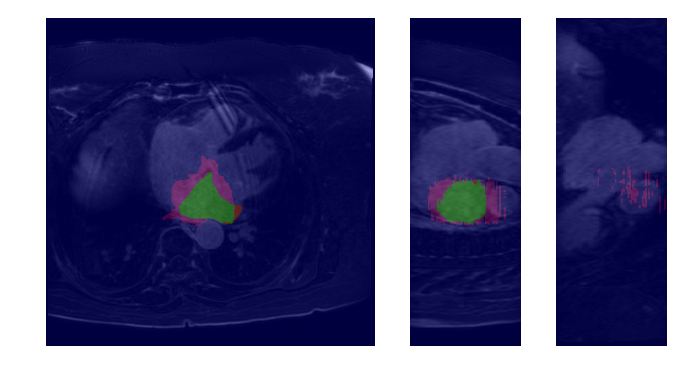
\includegraphics[trim=0cm 2cm 0cm 2cm, clip=true, height=50mm, width=75mm]{Chapter3/img/Masks_for_14022801.png}
\end{minipage}\hfill
\begin{minipage}{0.45\textwidth}
\centering
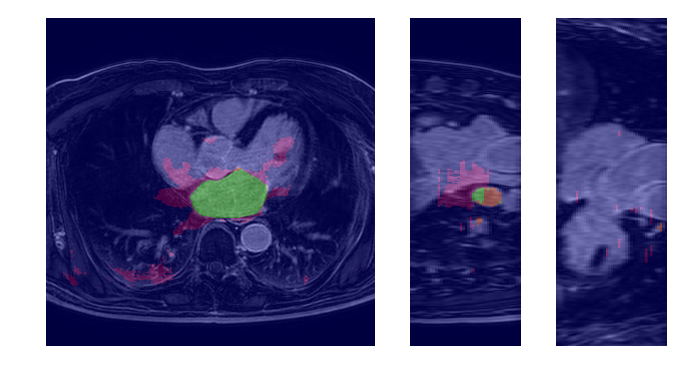
\includegraphics[trim=0cm 2cm 0cm 2cm, clip=true, height=50mm, width=75mm]{Chapter3/img/Masks_for_14012303.png}
\end{minipage}
\caption{Left: grey scale slices from a CT scan taken in the transversal, saggital and coronal planes. Right: illustration of the triplanar}
\label{final_model}
\end{figure}

\noindent Despite a good overall testing accuracy, the CNN behaves erratical on some of the masks observed. Figure \ref{final_model} shows 2 examples of such masks in the transversal, saggital and corronal planes taken at index 200, 200 and 20 on 2 different test CT scans. The masks on the left hand side show expected errors near the border regions of the atrium. The masks on the right hand side show more unexpected errors away from the atrium. More examples of masks taken from each of the test CT scans are shown in the Appendix.




















%\chapter{Conclusions and Further Work}

\noindent We conclude this thesis with a brief summary. We first discussed the recent advances which have allowed Deep Learning techniques to engender a string successes in pattern recognition, and particularly in the context of images. These successes have led to an increasing interest in applying these techniques to Medical Imaging. In the second chapter, we presented some background material on CNNs, covering convolutional layers, subsampling layers and an overview of the architectural organisation. In Chapter 3, we turn our attention to implementing a CNN ourselves using a tri-planar approach to generate the input set as a way of providing 3D information at a much lower cost than 3D patches along with a number of other practical considerations. We then performed model selection, finding a much better architecture and set of learning parameters than was initially proposed. To that end, we varied the number of convolutional and connected layers, the number of feature maps and hidden units, the type of activation function, the learning rate and the momentum. We then tried a different sampling procedure to increase the frequency of examples near the boundary of the atrium where most of the errors lie, yielding a significant increase in accuracy. Our final model gives a mean Dice coefficient of 0.985 across our 7 test CT scans. Most of the errors were at the border regions with the atrium where we expect them to be. However, despite the high rate of accuracy, the sensitivity was shown to be variable and some masks demonstrated errors far away from the atrium which we would expect the classifier not to commit. As a result, we do not expect this particular classifier to be useful for practicing radiologists in their work.\\

\noindent A number of things could be undertaken to improve the results. A first obvious step would be to increase the number of training examples. Another one would be to further improve with the sampling procedure in order to increase the number of training examples at the border regions. One could, for instance, systematically include all the pixels located at the border region of the atrium from each CT scan allocated to generating the training set. Another avenue for improvement would be to add more inputs channels to provide more information to the network, such as 3D patches.
%\include{Chapter5}

\end{document}